\documentclass[12pt]{article}

\usepackage{amsmath, amsfonts, amssymb}
\usepackage{graphicx}

\usepackage{epstopdf}

\begin{document}

\section{Introduction}

This is code for the registration and ordering algorithms described in \\
``Temporal ordering and registration of images in studies of developmental dynamics,'' Carmeline~J.~Dsilva, Bomyi~Lim, Hang~Lu, Amit~Singer , Stanislav~Y.~Shvartsman, and Ioannis~G.~Kevrekidis

The code reads in a set of two-dimensional images or three-dimensional z-stacks, can perform a number of preprocessing operations, and then registers and/or orders the images using the algorithms described in the paper. 

\section{Requirements}

All algorithms and analysis were implemented in MATLAB\textsuperscript{\textregistered} (R2013b, The MathWorks, Natick, Massachusetts).
%
The code requires MATLAB along with the Image Processing Toolbox. 

\section{How To Use}

There are two ways to use the code
\begin{enumerate}
\item Interactive GUI.
\item Program a simple script.
\end{enumerate}

The basic steps are as follows:
\begin{enumerate}
   \item Read in images
   \item Preprocess the images (smooth and/or equalize channels, mean-center, etc.)
   \item Run vector diffusion maps to register and order preprocessed images
   \item (Optional) Save registered and ordered images
\end{enumerate}

\subsection{Interactive GUI}

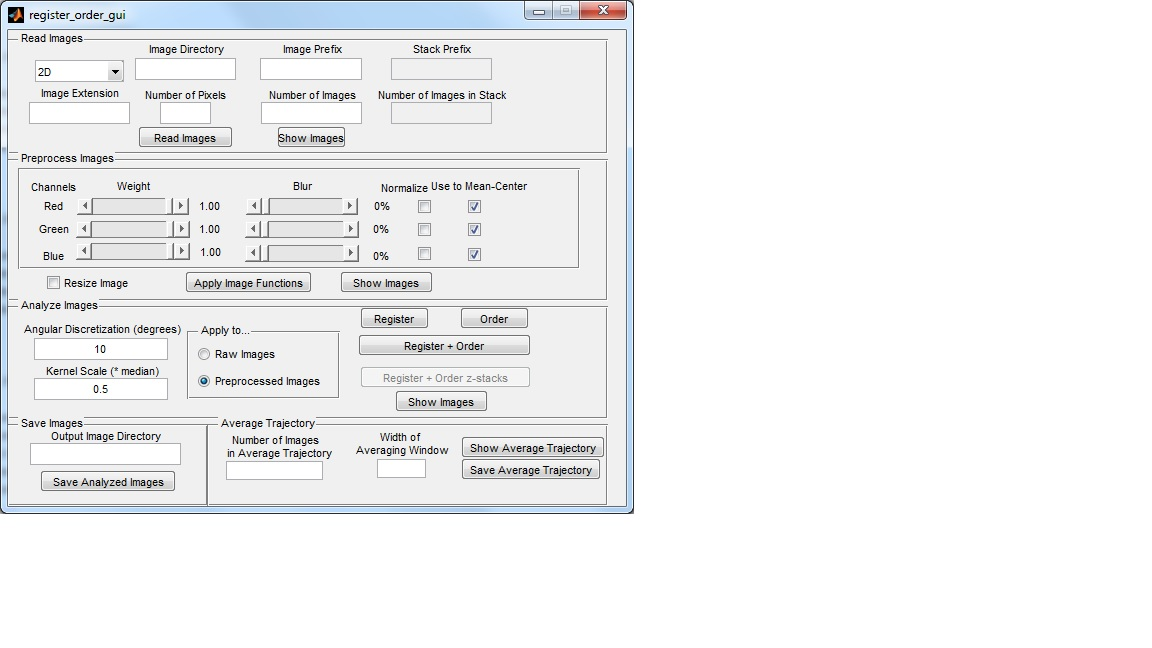
\includegraphics[width=10cm, trim=0cm 2cm 5cm 0cm, clip]{gui_screenshot_initial.jpg}

There are five steps
%
\begin{enumerate}
\item Read Images
\item Preprocess Images
\item Analyze Images
\item Save Images
\item Average Trajectory
\end{enumerate}

\subsubsection{Read Images}

The fields are as follows
\begin{description}
\item[2D/3D] Select ``2D'' if your images are traditional 2D images. Select ``3D'' if your images are z-stacks.
%
\item[Image Directory] Enter the directory where your images or z-stacks are stored. This directory can be an absolute path (e.g. \texttt{C:/Documents/Images}) or a path relative to the directory where this code is stored (e.g. \texttt{../images})
%
\end{description}
\subsection{Script}

\subsection*{Read Images}

\begin{par}
The first step is to read in images. This is done using the \texttt{read\_images} function For two-dimensional images, it requires that all the images are stored in a single directory, all with a consistent prefix, and indexed with two digits starting from \texttt{01}. For three-dimensional z-stack, it assumes each z-stack is stored in a single directory. All of the z-stack directories are required to begin with a consistent prefix, and be indexed with two digits starting from \texttt{01}. Similarly, all of the images are required to begin with a consistent prefix, and be indexed with two digits starting from \texttt{01} for each z-stack.
\end{par} \vspace{1em}
\begin{verbatim}
% directory where images are stored
image_dir = 'drosophila_fixed_images';

% prefix for each image
image_name = 'emb';

% image type/extension
image_ext = 'tif';

% no stack name or number of iamges in a stack are required for 2D images
stack_name = '';
nstack = 0;

% number of images
nimages = 120;

% number of pixels
npixels = 100;

% dimension of images (dim=2 indicates standard 2D images, rather than
% z-stacks)
dim = 2;

% read in images
% images are stored in the variable images_raw
[images_raw, nchannels] = read_images(image_dir, image_name, image_ext, ...
    stack_name, nimages, nstack, npixels, dim);
\end{verbatim}


\subsection*{Show images}

\begin{par}
An optional step is to now show the images using the \texttt{plot\_images} function.
\end{par} \vspace{1em}
\begin{verbatim}
% plot the images
% images_raw are the images to plot
% (returned from the read_images function)
% dim is the dimension of the images
% (dim=2 indicates standard 2D images, rather than z-stacks)
plot_images(images_raw, dim)
\end{verbatim}

\includegraphics [width=4in]{sample_input_file_01.eps}


\subsection*{Preprocess Images}

\begin{par}
Now, we must preprocess the images before registration and ordering, to remove any imaging and/or experimental artifacts. We do this via the \texttt{apply\_image\_functions} function For this particular imaging data set, there are three channels. DAPI, a nuclear stain, is in the first (red) channel. dpERK is in the second (green) channel. Dl is in the third (blue) channel.
\end{par} \vspace{1em}
\begin{verbatim}
% channel weights
% because the nuclear signal is wider spread throughout the image, as well
% as noiser, we choose to scale the first channel by half
channel_weight = [0.5 1 1];

% we blur the image slightly (5%) so that small-scale effects of individual
% nuclei are smoothened
channel_blur = [0.05 0.05 0.05];

% because the absolute intensity of the nuclear signal is not informative
% or important (only the presence or absence of signal is important,
% indicating the presence or absence of nuclei), we normalize the first channel
% We do not normalize the other two channels, as changes in intensity are
% informative to the developmental processes.
channel_normalize = [1 0 0];

% we use the nuclear channel to mean center the images, as this channel
% parameterizes/captures the entire embryo
channel_mean_center = [1 0 0];

% we resize the images to all be (approximately) the same size, to remove
% any variations due to size effects, as size effects are known to not be
% important for this developmental system
resize_image = true;

% we then apply these image functions of normalization, blurring,
% reweighting, and mean-centering
images = apply_image_functions(images_raw, dim, channel_weight, ...
    channel_blur, channel_normalize, channel_mean_center, resize_image);

% plot the images (optional)
plot_images(images, dim)
\end{verbatim}

\includegraphics [width=4in]{sample_input_file_02.eps}


\subsection*{Calculate pairwise alignments}

\begin{par}
We now need to calculate the angles needed to align \textit{pairs} of images
\end{par} \vspace{1em}
\begin{verbatim}
% angular discretization when computing pairwise aligments
% this means we search for pairwise aligmemnts over 10 degree increments
ang_dis = 10;

% compute the pairwise alignments
% images are the preprocessed images
% ang_dis is the angular discretization
% R and W store the pairwise alignments and distances, respectively, for
% vector diffusion maps
[R, W] = compute_pairwise_alignments(images, ang_dis);
\end{verbatim}


\subsection*{Apply vector diffusion maps}

\begin{par}
We can now use vector diffusion maps to register and order the images.
\end{par} \vspace{1em}
\begin{verbatim}
% ncomps is the number of components to compute
% we only compute 1 coordinate because we only need to order the images
% (i.e., sort by the first coordinate)
ncomps = 1;

% epsilon scale for diffusion maps kernel
% eps_scale = 0.25 means that the epsilon in the diffusion maps kernel is
% 1/4 of the median of the pairwise distances between data points
eps_scale = 0.25;

% vector diffusion maps calculates optimal rotations and embedding
% coordinate
[R_opt, embed_coord, D2] = vdm(R, W, eps_scale, ncomps);

% register images
images_registered = register_all_images(images, R_opt);

% order registered images by embedding coordinate
images_analyzed = order_all_images(images_registered, embed_coord);

% plot the images (optional)
plot_images(images_analyzed, dim)
\end{verbatim}

\includegraphics [width=4in]{sample_input_file_03.eps}


\end{document}

